\documentclass[12pt,a4paper]{article}

% ---------- 基础设置 ----------
\usepackage[utf8]{inputenc}
%\usepackage{ctex}              % 中文支持（如不需要可删）
\usepackage{geometry}          % 页面边距
\usepackage{graphicx}
\usepackage{hyperref}
\usepackage{amsmath,amssymb}
\usepackage{enumitem}
\usepackage{fancyhdr}
\usepackage{xcolor}
\usepackage{enumitem}
\usepackage{amssymb}
\usepackage{subcaption}

% ---------- 页面与格式 ----------
\geometry{margin=1in}
\setlength{\parskip}{0.75em}
\setlength{\parindent}{0em}
\renewcommand{\baselinestretch}{1}   % 行距
\pagestyle{fancy}
\fancyhf{}
\rfoot{\thepage}
\renewcommand{\normalsize}{\fontsize{12pt}{15pt}\selectfont}


% ---------- 文档信息 ----------
\title{\textbf{INT305 Coursework 1}}
\author{Name: Ruiyang Wu \quad Student ID: 2257475 \\ Programme: Information and Computing Science}
\date{\today}

\begin{document}
	
	\maketitle
	\vspace{-1em}
	\noindent\rule{\textwidth}{0.4pt}
	
	For a training example $(x_i,y_i)$ with $K$ classes:\\
	$s=Wx_i=score\;vector\;s_j$ ($s_j$= predicted score for class $j$) 
	
	\subsection*{Task 1: SVM Loss (35’)}

	\textbf{1)}  
	Derive SVM loss $L_i^{SVM}$ for $x_i$; set $\Delta$ as the margin hyper-parameter. (1’) 
	
	\textbf{Answer:}\\
	For an example $(x_i,y_i)$, where $x_i$ is the feature vector and $y_i \in \{1,2,...,K\}$ is its class label, we have the score vector $s_j=Wx_i$. 
	
	We want the score of the right class $s_{y_i}$ is at least $\Delta$ (margin) higher than the wrong class $s_j$, i.e. $s_{y_i}\ge s_j + \Delta$. Therefore, we want:
	\begin{equation}
		s_j-s_{y_i} + \Delta \le 0,\; \forall j\ne y_i
	\end{equation}

	In the case that the score of the right class $s_{y_i}$ is $\Delta$ (points) higher than the wrong class $s_j$, the classifier is correct and receives no penalty, which means: 
	\begin{equation}
	Loss = 0
	\end{equation}

	Otherwise the classifier is incorrect and will be penalized in proportion to how much it violates:
	\begin{equation}
		Loss = s_j-s_{y_i} + \Delta
	\end{equation}

	Thus, by adopting the hinge loss and considering $(2) \& (3)$, the Multi-class SVM loss for $x_i$ is:
	\begin{equation}
	L_i^{SVM} = \sum_{j\ne y_i} \max (0, s_j - s_{y_i} + \Delta)
	\end{equation}

	---
	
	\textbf{2)}  
	Derive the gradient $\frac{\partial L_i^{SVM}}{\partial s_k}$ for
	\begin{itemize}[itemsep=0pt, topsep=0pt, parsep=0pt, partopsep=0pt]
		\item $k = y_i$ (correct class) (5’)
		\item $k \ne y_i$ (incorrect class) (5’)
	\end{itemize}
	And explain:
	\begin{itemize}[itemsep=0pt, topsep=0pt, parsep=0pt, partopsep=0pt]
		\item why is $\Delta$ only applied to incorrect classes? (3’)
		\item How does $\Delta$ enforce a ``safety margin"? (5’)
	\end{itemize}
	
	\textbf{Answer:}\\
	Set $m_j = s_j - s_{y_i} + \Delta$, we have:
	\begin{equation}
		L_i^{SVM} = \sum_{j\ne y_i} \max (0, m_j)
	\end{equation}
	Let $g(u)=\max (0,u)$, the gradient of it (non-differentiable at 0, we take 0 here):
	\begin{equation}
		g'(u)=
		\left\{\begin{matrix}
			1,\; u>0
			\\
			0,\; u\le 0
		\end{matrix}\right.
	\end{equation}
	\textbf{1. In the case $k = y_i$ (correct class)}
	\begin{align}
		\frac{\partial L_i^{SVM}}{\partial s_k}&=\frac{\sum_{j\ne y_i} \max (0, m_j)}{\partial s_{k}}
		\\
		\because\;& every \; m_{j\ne y_i} \; contain \; (-s_{y_i})
		\\
		\therefore &=\sum_{j\ne y_i} g'(m_j)\cdot (-1)
		\\
		&=-\sum_{j\ne y_i}1\cdot [s_k - s_{y_i}+\Delta >0]
	\end{align}

	\textbf{2. In the case $k \ne y_i$ (incorrect class)}
	\begin{align}
		\frac{\partial L_i^{SVM}}{\partial s_k}&=\frac{\sum_{j\ne y_i} \max (0, m_j)}{\partial s_{k}}
		\\
		\because\;& only \; m_{j=k} \; contains \; s_k
		\\
		\therefore &=g'(m_k)\cdot 1
		\\
		&=1\cdot [s_k - s_{y_i}+\Delta >0]
	\end{align}
	
	\textbf{3. Why is $\Delta$ only applied to incorrect classes:}
	$\Delta$ is a hyper-parameter in order to control the difference of the scores between correct and incorrect classes. As I mentioned in (1), $\Delta$ plays the role of relative gap (or margin) between 2 classes, so there is no need to apply it towards both sides of the equation, or they will be eliminated! 
	
	\textbf{4. How does $\Delta$ enforce a ``safety margin":}
	If there is no $\Delta$, i.e. $\Delta = 0$, our model only try to maximize the score of correct classifications; when $\Delta > 0$, model need to ensure the score of correct class is at least $\Delta$ scores higher than the incorrect ones. Higher the $\Delta$ is, wider the ``safety margin" is. Making the model more robust against the noise and promotes better generalization performance.
	
	---
	
	\textbf{3)}  
	Given scores $s = [3,-1,4]$ for classes [``cat",``dog",``bird"]; True class $y_i$ is ``cat" (index = 0); $\Delta = 1$, compute and explain:
	\begin{itemize}[itemsep=0pt, topsep=0pt, parsep=0pt, partopsep=0pt]
		\item $L_i^{SVM}$ for each score (3’)
		\item How does $L_i^{SVM}$ change if $\Delta = 2$? (5’)
	\end{itemize}
	
	\textbf{Answer:}\\
	\textbf{1. $L_i^{SVM}$ for each score:}
	\begin{align}
		j=1\;(Score \; of \; ``dog"):\; &\max(0, s_1-s_0+\Delta)
		\\
		=&\max(0,-1-3+1)=\max(0,-3)=0
		\\
		j=2\;(Score \; of \; ``bird"):\; &\max(0, s_2-s_0+\Delta)
		\\
		=&\max(0,4-3+1)=\max(0,2)=2
		\\
		\therefore L_i^{SVM}=&\sum_{j\ne y_i}\max(0,s_j-s_{y_i}+\Delta)
		\\
		=&0+2=2
	\end{align}
	\textbf{2. How does $L_i^{SVM}$ change if $\Delta = 2$:}
	\begin{align}
		j=1\;(Score \; of \; ``dog"):\; &\max(0, s_1-s_0+\Delta)
		\\
		=&\max(0,-1-3+2)=\max(0,-2)=0
		\\
		j=2\;(Score \; of \; ``bird"):\; &\max(0, s_2-s_0+\Delta)
		\\
		=&\max(0,4-3+2)=\max(0,3)=3
		\\
		\therefore L_i^{SVM}=&\sum_{j\ne y_i}\max(0,s_j-s_{y_i}+\Delta)
		\\
		=&0+3=3\; wow \; it \; increased\; by\; 1!
	\end{align}
	
	---
	
	\textbf{4)}  
	Using the same score $s = [3,-1,4]$ and $y_i = 0$:
	\begin{itemize}[itemsep=0pt, topsep=0pt, parsep=0pt, partopsep=0pt]
		\item Compute $\frac{\partial L_i^{SVM}}{\partial s}$ (3’)
		\item Interpret the gradient: Why are some values positive, negative, or zero? (5’)
	\end{itemize}
	
	\textbf{Answer:}\\
	\textbf{1. Compute:}
	\begin{align}
		\frac{\partial L_i^{SVM}}{\partial s}&=\frac{\partial \sum_{j\ne 0}\max(0,s_j-s_0+1)}{\partial s}
		\\
		ignore\;j=1&,\;no\;active\; (see\; (22)): 
		\\
		&=(\frac{\partial \max(0,s_2-s_0+1)}{\partial s_0},\frac{\partial \max(0,s_2-s_0+1)}{\partial s_1},\frac{\partial \max(0,s_2-s_0+1)}{\partial s_2})
		\\
		&=(\frac{\partial (s_2-s_0+1)}{\partial s_0},\frac{\partial (s_2-s_0+1)}{\partial s_1},\frac{\partial (s_2-s_0+1)}{\partial s_2})
		\\
		&=(-1,0,1)
	\end{align}
	\textbf{2. Why are some values positive, negative, or zero:} Incorrect class ``bird" ($j=2$) activates the hinge, so its gradient becomes positive, pushing $s_2$ descend; therefore correct class ``cat" ($j=0$) becomes negative (simply take the derivative), pushing $s_0$ ascend; ``dog" ($j=1$) did not activate the hinge, so its gradient is zero.

	---
	
	\section*{Task 2: Softmax Loss (35’)}
	
	\textbf{1)}  
	Derive
	\begin{itemize}[itemsep=0pt, topsep=0pt, parsep=0pt, partopsep=0pt]
		\item Softmax probability $p_j$ for class $j$ (1’)
		\item Softmax loss $L^{softmax}_i$ (1’)
	\end{itemize}

	\textbf{Answer:}\\
	\textbf{1. Softmax probability $p_j$ for class $j$:}
	\begin{align}
		p_j&=\frac{e^{s_{j}}}{\sum_{n=1}^K e^{s_n}}
	\end{align}
	\textbf{2. Softmax loss $L^{softmax}_i$:}
	\begin{align}
		L^{softmax}_i&=-\log_e(\frac{e^{s_{y_i}}}{\sum_{j} e^{s_j}}) = -s_{y_i}+\log \sum_j e^{s_j}
	\end{align}

	---
	
	\textbf{2)}  
	Derive the gradient $\frac{\partial L_i^{softmax}}{\partial s_k}$ for
	\begin{itemize}[itemsep=0pt, topsep=0pt, parsep=0pt, partopsep=0pt]
		\item $k = y_i$ (correct class) (5’)
		\item $k \ne y_i$ (incorrect class) (5’)
	\end{itemize}
	And explain:
	\begin{itemize}[itemsep=0pt, topsep=0pt, parsep=0pt, partopsep=0pt]
		\item Why does minimizing $L_i^{softmax}$ force $p_{y_i}\rightarrow 1$? (3’)
	\end{itemize}

	\textbf{Answer:}\\
	\textbf{1. In the case $k = y_i$ (correct class):}
	\begin{align}
		\frac{\partial L_i^{softmax}}{\partial s_k}&=(-s_{y_i}+\log \sum_j e^{s_j})\frac{\partial}{\partial s_{y_i}}
		\\
		&=p_{y_i}-1
	\end{align}
	\textbf{2. In the case $k \ne y_i$ (incorrect class):}
	\begin{align}
		\frac{\partial L_i^{softmax}}{\partial s_k}&=(-s_{y_i}+\log \sum_j e^{s_j})\frac{\partial}{\partial s_{k}}
		\\
		&=p_{k}
	\end{align}
	\textbf{3. Why does minimizing $L_i^{softmax}$ force $p_{y_i}\rightarrow 1$:} From the view of gradient, because $\forall \; p_k\in(0,1)\; s.t. \frac{\partial L_i^{sm}}{\partial s_{y_i}}=p_{y_i}-1<0,\; \frac{\partial L_i^{sm}}{\partial s_{k\ne y_i}}=p_{k}>0$ Therefore, in the case where there is no constraint during the process of gradient descent, $p_{y_i}$ will monotonically increase, the limit tends towards 1; meanwhile $p_{k}$ will monotonically decrease.
	
	---
	
	\textbf{3)}  
	Given scores $s = [3,-1,4]$ for classes [``cat",``dog",``bird"]; True class $y_i$ is ``cat" (index = 0), compute and explain:
	\begin{itemize}[itemsep=0pt, topsep=0pt, parsep=0pt, partopsep=0pt]
		\item $p_j$ (3’)
		\item $L_i^{softmax}$ for the given scores (3’)
		\item What happens to $L_i^{softmax}$ if all scores are scaled by 2 (i.e., $s_{new}=2s$) (4’)
	\end{itemize}
	
	\textbf{Answer:}\\
	\textbf{1. Compute $p_j$:}
	\begin{align}
		e^{s_0}&=e^3 \approx 20.086,\; e^{s_1}=e^{-1} \approx 0.36788,\; e^{s_2}=e^4 \approx 54.598,\;\sum_j e^{s_j}\approx 75.052
		\\
		p_0&=\frac{e^{s_0}}{\sum_j e^{s_j}} \approx \frac{20.086}{75.052} \approx 0.26763,\; 
		p_1=\frac{e^{s_1}}{\sum_j e^{s_j}} \approx \frac{0.36788}{75.052} \approx 0.0049,\\
		p_2&=\frac{e^{s_2}}{\sum_j e^{s_j}} \approx \frac{54.598}{75.052} \approx 0.72747
	\end{align}
	\textbf{2. Compute $L_i^{softmax}$:}
	\begin{align}
		L_i^{softmax}= -\log_e(p_0)\approx1.3181
	\end{align}
	\textbf{3. What happens to $L_i^{softmax}$ if all scores are scaled by 2:}  $s_{new} = [6,-2,8]$
	\begin{align}
		e^6&\approx403.4,\;e^{-2}\approx0.1353,\;e^8\approx2980,\; \sum_j e^{s_j}\approx 3384
		\\
		p_0&\approx0.1192,\;p_1\approx0.00004,\;p_2\approx0.8806
		\\
		L_i^{softmax}&= -\log_e(p_0)\approx2.127
	\end{align}
	When the correct class is not the highest score, scaling up will enhance the relative difference, concentrate the probability to the highest score class (in this case, ``bird"), thereby increasing the loss.
	
	In other circumstances, if the correct class got the highest score, scaling up may reduce the loss.
	
	---
	
	\textbf{4)}  
	Using the same score $s = [3,-1,4]$ and $y_i = 0$:
	\begin{itemize}[itemsep=0pt, topsep=0pt, parsep=0pt, partopsep=0pt]
		\item Compute $\frac{\partial L_i^{Softmax}}{\partial s}$ (3’)
		\item How does the gradient for the correct class differ from SVM? (7’)
	\end{itemize}
	
	\textbf{Answer:}\\
	\textbf{1. Compute:} From Task 2.2:
	\begin{align}
		\frac{\partial L_i^{Softmax}}{\partial s_0}&= p_0-1\approx -0.7324
		\\
		\frac{\partial L_i^{Softmax}}{\partial s_1}&= p_1\approx 0.0049
		\\
		\frac{\partial L_i^{Softmax}}{\partial s_2}&= p_2\approx 0.7275
		\\
		\therefore \frac{\partial L_i^{Softmax}}{\partial s}&\approx (-0.7324, 0.0049, 0.7275)
	\end{align}
	\textbf{2. How does the gradient for the correct class differ from SVM:}
	Softmax provides a soft and probabilistic adjustment, while SVM is harder (0/1).
	\begin{align}
		\frac{\partial L_i^{softmax}}{\partial s_{y_i}} = p_{y_i} - 1, \qquad
		\frac{\partial L_i^{SVM}}{\partial s_{y_i}} = -\sum_{j\ne y_i}\mathbf{1}[s_j - s_{y_i} + \Delta > 0]
	\end{align}
	Focus on the correct class, the Softmax gradient changes smoothly: it goes from -1 when $p_{y_i}$ is small to 0 as $p_{y_i}\to1$. The higher the probability, the weaker the model push.
	While the gradient of SVM is discrete constant: it stays negative until all margins are satisfied, then turn to 0.
	
	---
	
	\section*{Task 3:  Comparative Analysis (30’)}
	Before getting into the details, let me use two plots to show the relationship of magnitude and gradient between SVM loss (with $\Delta=1$) and Softmax loss as the function of relative margin:
	\begin{figure}[h]
		\centering
		\begin{subfigure}{0.49\textwidth}
			\centering
			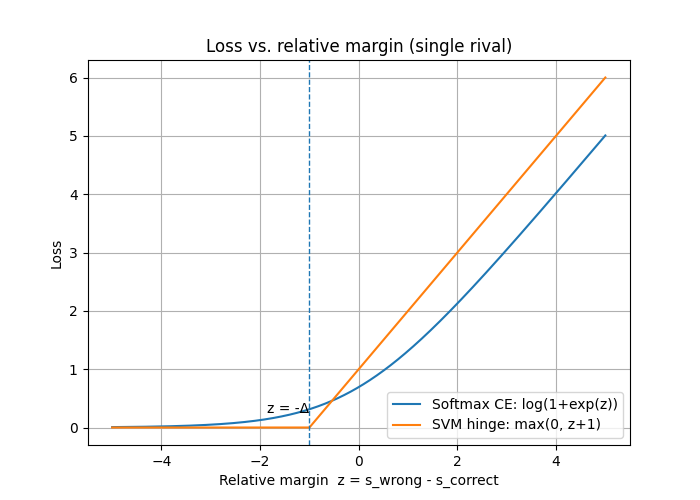
\includegraphics[width=\linewidth]{myplot1.png}
			\caption{Loss vs. Relative margin}
			\label{fig:sub1}
		\end{subfigure}
		\hfill
		\begin{subfigure}{0.49\textwidth}
			\centering
			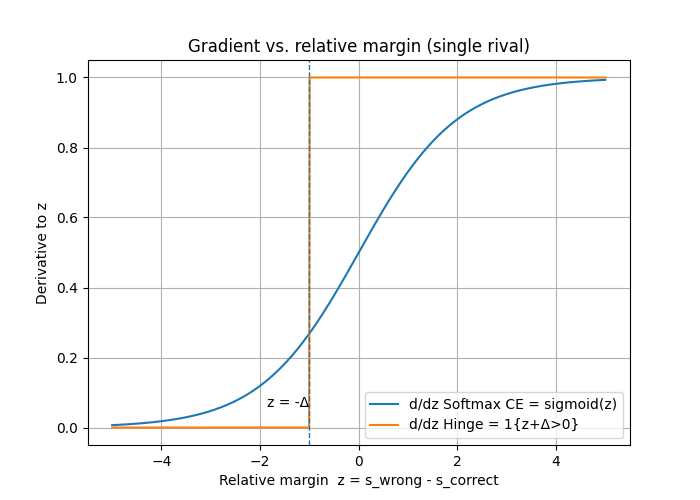
\includegraphics[width=\linewidth]{myplot2.png}
			\caption{Gradient vs. Relative margin}
			\label{fig:sub2}
		\end{subfigure}
		\caption{Comparison of $L_i^{SVM}$ and $L_i^{Softmax}$}
		\label{fig:twopics}
	\end{figure}
	
	\textbf{1)}  
	Using the same score $s = [3,-1,4]$ and $y_i = 0$:
	\begin{itemize}[itemsep=0pt, topsep=0pt, parsep=0pt, partopsep=0pt]
		\item Compare the previous derived losses $L_i^{SVM}$ and $L_i^{Softmax}$, which is larger? (2’)
		\item Why? (3’)
	\end{itemize}

	\textbf{Answer:}\\
	\textbf{1. Compare:} $L_i^{SVM}$ is larger than $L_i^{Softmax}$.
	\begin{align}
		L_i^{SVM}=2\; (see\; (20))\; > L_i^{Softmax}\approx 1.3181(see\; (44))
	\end{align}
	\textbf{2. Why:}\\
	In this case, there is 1 incorrect class outside the margin (i.e., $s_2 - s_y=1$). As you can see in Fig.1(a). The SVM Loss (Hinge) penalizes this linearly with margin $\Delta$:
	\begin{align}
		L_i^{SVM}=1+\Delta=2
	\end{align}
	While the Softmax Loss (Cross Entropy) focus on the allocation of probability $(p_0\approx26.8\%, p_1\approx0.5\%, p_2\approx72.7\%)$, it uses log-sum-exp, which compresses large gaps and spreads penalty across all classes by their probabilities:
	\begin{align}
		L_i^{Softmax}=-\log_e\frac{e^3}{e^3+e^{-1}+e^4}=\underbrace{\log_e\{1+e^{(-1-3)}+e^{(4-3)}\}}_{grow\; sublinearly}\approx 1.318
	\end{align}
	Therefore, in this case the $L_i^{SVM}$ is larger than $L_i^{Softmax}$.
	
	* Please notify that when there is little violation (see Fig.1(a)), it is possible for Softmax Loss become higher than SVM Loss, encouraging higher confidence.
	
	---
	
	\textbf{2)}
	Using the gradients from task1 and task2:
	\begin{itemize}[itemsep=0pt, topsep=0pt, parsep=0pt, partopsep=0pt]
		\item How does SVM penalize ``near-miss" errors (e.g., $s_j\approx s_{y_i}$) vs. ``large-margin" errors? (2’)
		\item How does Softmax adjust probabilities for low-confidence predictions? (3’)
	\end{itemize}
	
	\textbf{Answer:}\\
	\textbf{1. How does SVM penalize:}\\
	As you can see in Fig.1(b), the ``Red line" is $s_{y_i} - \Delta$. For the ``near-miss" errors (e.g., $s_j\approx s_{y_i}$), once $s_j>s_{y_i} - \Delta$, the hinge loss turns on and grows linearly; but for the samples who did not cross the ``Red line", there is no penalty. For the ``large-margin" errors, the loss still increases linearly.
	
	In other words, SVM Loss does not scale the gradient with “how badly” a class violates the margin. Every active violator gets the same push, no matter it is ``totally wrong" or ``nearly right".
	
	\textbf{2. How does Softmax adjust probabilities:}\\
	When the confidence is low ($0< p_{y_i}\ll 1$), the correct class gets a strong negative gradient ($(p_{y_i}-1)\approx -1$), strongly lifting $s_{y_i}$. 
	Meanwhile, each wrong class get positive gradient with proportional to their probabilities, higher penalty to higher probability class. Finally, as $p_{y_i}\to 1$, gradients decrease smoothly to 0 (see Fig.1(a)).
	
	Hence, Softmax is probability-aware and smooth, allocating larger updates to the most confusing wrong classes.
	
	---
	
	\textbf{3)}  
	Why is SVM loss called ``max-margin" and Softmax ``cross-entropy"? Please use your own words to define them and show your understanding of the definition and meaning of them. (8')
	
	\textbf{Answer:}\\
	\textbf{1. Why does SVM loss called ``max-margin":}\\
	\begin{equation}
		L_i^{SVM} = \sum_{j\ne y_i} \max (0, s_j - s_{y_i} + \Delta)
	\end{equation}
	We want the score of the right class $s_{y_i}$ is at least $\Delta$ higher than the wrong class $s_j$, the margin hyper-parameter $\Delta$ controls the width of the margin. It only care about the class which beyond the margin and gives linear penalty, otherwise the loss is 0.
	
	During the training procedure, SVM Loss trying to minimize the violation (i.e., $s_{y_i}\ge s_j+\Delta$). Geometrically maximizes the minimum margin between classes: a larger margin ($\frac{1}{||W||}$), which makes the model more robust against the noise and promotes better generalization performance. This is why I think SVM loss is called ``max-margin".
	
	\textbf{2. Why does Softmax loss called ``cross-entropy":}\\
	Firstly, let me introduce ``cross-entropy". In the Information Theory, suppose we have 2 distribution: $q$, $p$ represent for the target and predicted distribution respectively, the ``distance" between two distribution (i.e., cross-entropy) is defined as:
	\begin{equation}
		H(q,p)=-\sum_k q_k\log_e p_k
	\end{equation}
	In the circumstance of supervised classification with one-hot labels, we have $q_k=1,\; k=y_i$:
	\begin{align}
		\Rightarrow H(q,p)&=-\log_e p_{y_i} \qquad p_{y_i}=\frac{e^{s_{y_i}}}{\sum_{n=1}^K e^{s_n}}=softmax(s_{y_i})
		\\
		\therefore H(q,p)&=-\log(softmax(s_{y_i})) =L_i^{Softmax}
	\end{align}
	Clearly, they are the same. What's more, since $H(q,p)=\underbrace{H(q)}_{constant}+D_{KL}(q||p)$, minimizing the Softmax cross-entropy is equivalent to maximum likelihood estimation (MLE) or minimizing $D_{KL}(q||p)$.

	---
	
	\textbf{4)}  
	Compare between SVM loss and Softmax loss, which is better and why? (in this case, please not just focus on previous tasks and show your understanding of the two losses) (12’)
	
	\textbf{Answer:} I think it depends, the better choice depends on the application goal: Softmax is generally fit for probability modeling and smooth optimization, while explicit geometric margins and sparse updates often prefer SVM loss.
	
	\medskip
	\textbf{1. The philosophy of each goal:}
	Softmax cross-entropy treats logits $s=(s_1,\dots,s_K)$ as a categorical model with probabilities $p_k=\frac{e^{s_k}}{\sum_j e^{s_j}}$ and minimizes $L_i^{\text{Softmax}}=-\log p_y=-s_y+\log\!\sum_{j}e^{s_j}$
	i.e., maximum likelihood; SVM hinge loss with margin $\Delta>0$, $L_i^{\text{svm}}=\sum_{j\neq y}\max\{0,\ s_j-s_y+\Delta\}$ enforces large margins; with $\tfrac12\|W\|^2$ regularization it explicitly maximizes geometric separation.
	
	\medskip
	\textbf{2. Geometry and numerical shape:}
	With multiple rivals, softmax grows sublinearly according to their count due to the $\log\sum e^{z_k}$ compression, while hinge sums violations linearly. 
	Hinge is continuous but non-smooth (at $z=-\Delta$); softmax is smooth everywhere.
	
	\begin{figure}[h]
		\centering
		\begin{subfigure}{0.49\textwidth}
			\centering
			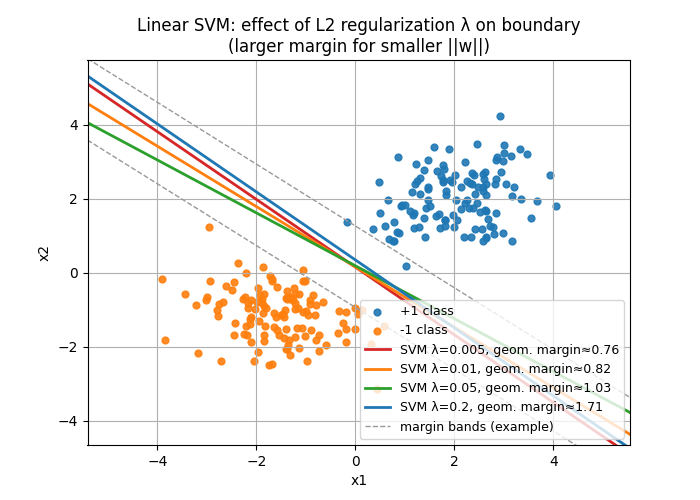
\includegraphics[width=\linewidth]{myplot3.png}
			\caption{SVM Loss}
			\label{fig:sub1}
		\end{subfigure}
		\hfill
		\begin{subfigure}{0.49\textwidth}
			\centering
			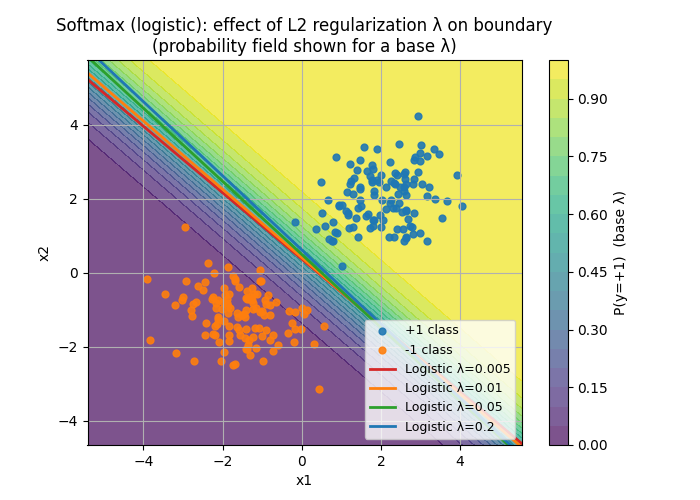
\includegraphics[width=\linewidth]{myplot4.png}
			\caption{Softmax}
			\label{fig:sub2}
		\end{subfigure}
		\caption{Geometry and numerical shape of $L_i^{SVM}$ and $L_i^{Softmax}$}
		\label{fig:twopics}
	\end{figure}

	\medskip
	\textbf{3. Gradient allocation:}\\
	Softmax has$\frac{\partial L}{\partial s_y}=p_y-1,\; \frac{\partial L}{\partial s_k}=p_k$
	so gradients are dense and confidence-aware: every wrong class gets a push proportional to $p_k$, and as $p_y\to 1$ all gradients decay smoothly.
	
	Hinge has $\frac{\partial L}{\partial s_y}=-\!\!\sum_{k\neq y}\mathbf{1}[z_k+\Delta>0],\;
	\frac{\partial L}{\partial s_k}=\mathbf{1}[z_k+\Delta>0],$
	so gradients are sparse and binary: only margin violators are updated (equally), and once safe, a sample gives zero signal.
	
	Softmax thus keeps optimizing the whole distribution; while hinge concentrates on hard points!
	
	\medskip
	\textbf{4. Probabilities, entropy, and calibration:}
	Softmax outputs probabilities and, via cross-entropy, reduces predictive entropy; it works naturally with label smoothing and we can use temperature scaling for calibration. SVM yields margins rather than probabilities.
	
	\medskip
	\textbf{5. Robustness against noise:}
	Softmax loss scales like $-\log p_y$; its gradients are bounded ($p_y-1\in[-1,0)$, $p_k\in(0,1)$), numerically stable but potentially sensitive to label noise without regularization (can be mitigated by smoothing/ early stopping/ clipping etc.). 
	Hinge grows linearly with violations and is exactly zero in the safe region—sometimes more tolerant to easy examples and certain outliers, but non-smoothness can slow optimization.
	
	\medskip
	\textbf{6. Optimization in practice:}
	Softmax is smooth and well-conditioned in logits, ideal for backprop in deep network. 
	Hinge is continuous but non-smooth; in deep settings hinge’s sparse/binary updates may converge slower than Cross Entropy’s dense, confidence-aware signals.
	
	\medskip
	\textbf{Which is better? It depends on the goal.}\\
	Choose Softmax CE if you need well-formed probabilities and strong log-loss performance, or if you are training deep networks where smooth, dense gradients help optimization. It is also preferred when the downstream metrics or decisions depend on calibrated probabilities, likelihood, ranking, or uncertainty estimates, and when stable gradient flow is needed.
	Use SVM loss when caring about explicit large margins, and want training to focus on hard negatives while ignoring already-safe points.
	
	The key idea is matching the loss to the evaluation target: if you evaluate likelihood/ calibration, use Cross Entropy; if you evaluate geometric separation/ margin, use hinge. 
	There is no one single loss fits all. In my experience, practically, during the implementation of machine learning model or deep neural network, we design the loss function that is corresponding to the learning objective and model structure; each part of loss encodes a coherent inductive bias that works when aligned with the problem’s objective.
	
	I believe this is the real beauty of machine learning and deep learning: When mathematics resonates with the structures we design, human endow machines with ``intelligence". From the innovation of very first data-driven algorithm to the LLMs (Large language models) with hundreds of billions of parameters nowadays, my friend, do not be fear of whether we are the modern ``Frankenstein". In the era of artificial intelligence, we are not the only ``Homo sapiens"!
	
	---
	
	\section*{Acknowledgments}
	Thank you for the thoughtful design of the coursework and your careful marking. The questions provided a clear way to examine core ideas in machine learning, and I have done my best to address them.
	
	Wish you a great day.
	
\end{document}
